\documentclass[11pt,a4paper]{article}
\usepackage[utf8]{inputenc}
\usepackage[T1]{fontenc}
\usepackage{mathptmx}
\usepackage{amsfonts}
\usepackage{amsmath, amssymb}
\usepackage{bm}
\usepackage{nccmath}
\usepackage{graphicx}
\usepackage{titling}
\usepackage{indentfirst}
\usepackage{url}
\usepackage{xurl}
\usepackage[backend=biber,style=apa,date=year]{biblatex}
\usepackage{csquotes}
\usepackage{float}
\usepackage{sectsty}
\usepackage{enumitem}
\usepackage{hyphenat}
\usepackage{wrapfig}
\usepackage{hyperref}
\usepackage{enumitem}
\usepackage{titlesec}
\usepackage{authblk}
\usepackage[skip=0pt]{caption}
\DeclareSourcemap{
  \maps[datatype=bibtex]{
      \map{
        \step[fieldset=urldate, null]
      }
   }
}
\usepackage[top=0.5in, bottom=0.5in,left=1in,right=1in]{geometry} 
\addbibresource{Bio.bib}

\DeclareMathSymbol{\mh}{\mathord}{operators}{`\-}
\renewcommand{\thetable}{S\arabic{table}}
\renewcommand{\thefigure}{S\arabic{figure}}
\renewcommand{\theequation}{S\arabic{equation}}
\renewcommand{\thesection}{SM\arabic{section}}

\date{}

\begin{document}

\begin{center}
\Large
Identifying robust adaptive irrigation operating policies to balance deeply uncertain economic food production and groundwater sustainability trade-offs \\ 
\vspace{0.5cm}
Supplementary Material
\end{center}

\begin{center}
José M. Rodríguez-Flores$^{1,*}$, Rohini S. Gupta $^2$, Harrison B. Zeff $^3$,\\ Patrick M. Reed $^2$, Josué Medellín-Azuara $^1$\\
\end{center}

\begin{center}
\small
$^1$Environmental Systems Program, University of California Merced, CA, USA\\
$^2$Department of Civil and Environmental Engineering, Cornell University, NY, USA\\
$^3$Department of Environmental Sciences and Engineering, University of North Carolina at Chapel Hill, NC, USA\\
$^*$Corresponding Author: jrodriguezflores3@ucmerced.edu
\end{center}

\vspace{0.2cm}

\section{Flexible Sustainable Groundwater Management}

The Sustainable Management Criteria (\cite{dwr_sustainable_2017}) defines:

\begin{itemize}
    \item Sustainable groundwater management as \textit{"the management and use of groundwater in a manner that can be maintained during the planning and implementation horizon without causing undesirable results."}
    \item Measurable objectives is \textit{"the specific, quantifiable goals for the maintenance or improvement of groundwater conditions that have been included in an adopted Plan."}
    \item The minimum threshold is \textit{"the quantitative value that represents the groundwater condition in each representative monitoring well site that when exceeded, may cause an undesirable result."}
\end{itemize}

\section{Economic Model Calibration}

We used a Positive Mathematic Programing (PMP) (\cite{howitt_calibration_1995}) calibration that employs a stochastic data assimilation process to calibrate the economic model (\cite{maneta_satellite-driven_2020}).  With this calibration we address two objectives: avoid the assumption that farmers will behave as a particular year or average of years but rather capturing the mid-term farmers behavior using all the data available from 1999 to 2015, and second, we account for the uncertainty in the calibration parameters inherited from uncertain inputs used in the calibration. This stochastic framework enables us to update the distribution of parameters as new observations become available. We adapted the Python code used by \textcite{maneta_satellite-driven_2020} that performs a Monte Carlo recursive Bayesian estimator based on the ensemble Kalman Filter (enKF) (\cite{evensen_sequential_1994}). The enKF uses uses the calibration conditions to recursively update the distribution of the parameters using historical data on crop production, land use, water use, own-price supply elasticities, crop yield response to water (elasticity) and production costs. The optimality conditions to perform the stochastic assimilation follow the PMP calibration described by \textcite{merel_fully_2011} which uses using a generalized Constant Elasticity of Substitution (CES) production function as a concave production function, and the calibration of the Lagrange multipliers used in the linear costs of land and water explained by  \textcite{garnache_calibration_2017}. 

The goal of the calibration stage is to replicate observed inputs allocation to crops and yield. Following the necessary and sufficient optimality conditions or Karush-Kuhn-Tucker conditions of the maximization problem (Equations S1) that are solved so the model calibration parameters can reproduce the observed allocation of inputs land and water per crop ($\tilde{x}_{i,land},\tilde{x}_{i,water}$).

\begin{align}
&\underset{{\substack{x_{i,land}\geq0\\x_{i,water}\geq0}}}{max} \sum_{i} \{p_{i}\mu_{i}(\beta_{i,land} x^{\rho_i}_{i,land}+\beta_{i,water} x^{\rho_i}_{i,water})^{\delta_{i}/\rho_i} - (\omega_{i,land}) x_{i,land}-(\omega_{i,water})x_{i,water}\}&\notag
\end{align}
\textit{subject to:}
\begin{align}
&\sum_{i} x_{i,land} \leq b_{land}[\bar{\lambda}_{land}]&\\
&x_{i,land} = \tilde{x}_{i,land}[\lambda_{i,land}]\notag\\
&x_{i,water} = \tilde{x}_{i,water}[\lambda_{i,water}]\notag
\end{align}

Where $\mu_{i},\beta_{i,water},\beta_{i,land},\delta_{i},\rho_i$ are the calibration parameters used the CES production function (\cite{merel_fully_2011}) and $\lambda_{i,land},\lambda_{i,water},\bar{\lambda}_{land}$ the Lagrange multipliers for the total land and crop-specific use of inputs restrictions. The crop-specific input use restriction guarantees that the solution will reproduce the observed input use. $p_i$ is the crop price per crop and $\omega_{i,land}$ and $\omega_{i,water}$ represent the average land and water costs.  For the case of water such cost is weighted by the proportion of surface and groundwater baseline use. Even though the economic model described in Section 2.1.1 solves for two sources of water (groundwater and surface water), the calibration was performed aggregating both sources of water. Calibration parameters and crop specific Lagrange multipliers are obtained for the crop groups $i\in$ \{Alfalfa, Almonds and Pistachios, Corn, Cotton, Cucurbits, Dry Beans, Fresh Tomatoes, Grain, Onions and Gralic, Other Deciduous, Other Field, Other Truck, Pasture, Processing Tomatoes, Safflower, Subtropical and Vine\} shown in Figure S1. 

\begin{figure}[htb!]
    \centering
    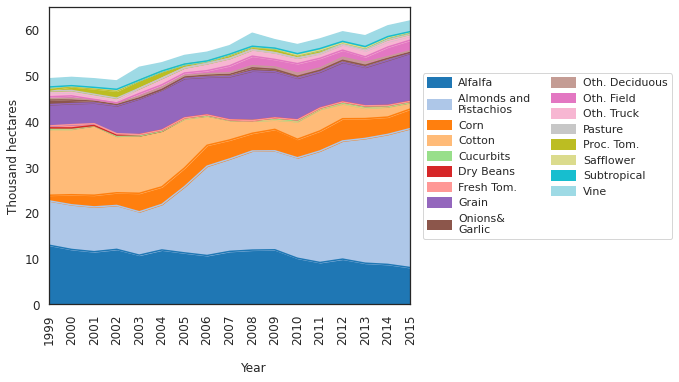
\includegraphics[width=0.7\textwidth]{./figs/land_hist_semitropic.png}
    \caption{Historical cropland of Semitropic WSD}
    \label{fig:S1}
\end{figure}

The PMP maximization problem defined by the set of Equations S1 can be formulated following its first order optimality conditions and arranged as a set of nonlinear equations as proposed by  \textcite{garnache_calibration_2017}. Where on the left-hand side of Equations S2 are the observed quantities and on the right-hand side are the model functions that include the parameters that we are estimating. 

\begin{flalign}
&-p_{i} \tilde{y_i} \tilde{y}_{i,water}= (\omega_{i,land}+\lambda_{i,land}+\bar{\lambda}_{land})\tilde{x}_{i,land}-p_{i}\tilde{y}_i\delta_{i}& \notag\\
&p_{i} \tilde{y_i} \tilde{y}_{i,water}=  (\omega_{i,water}+\lambda_{i,water})\tilde{x}_{i,water} \notag\\
&\tilde{\eta}_i = \dfrac{\delta_i}{1-\delta}  \left\{1-\dfrac{\dfrac{b_i}{\delta_i(1-\delta_i)}}{\sum_i[\dfrac{b_i}{\delta_i(1-\delta_i)}+\dfrac{\sigma_{i}b_{i}\tilde{y}_{i,water}}{\delta_i(\delta_i-\tilde{y}_{i,water})}]}\right\}, b_{i} = \dfrac{(\tilde{x}_{i,land})^2}{p_i \tilde{y}_{i}} \notag\\
&\tilde{y}_{i,water} = \delta_{i}(\dfrac{\beta_{i,water}(\tilde{x}_{i,land})^{\rho_i}}{\beta_{land,i}(\tilde{x}_{i,land})^{\rho_i}+\beta_{i,water}(\tilde{x}_{i,water})^{\rho_i}})\\
&\tilde{y}_{i}=\mu_{i}(\beta_{i,land} x^{\rho_i}_{i,land}+\beta_{i,water} x^{\rho_i}_{i,water})^{\delta_{i}/\rho_i} \notag\\
&\sum_{i} \{(2\tilde{x}_{i,land}p_{i}\tilde{y}_{i}\tilde{y}_{i,water})=\sum_i -2(\omega_{i,land}+\lambda_{land})(\tilde{x}_{i,land})^2 + 2\tilde{x}_{i,land}p_{i} \tilde{y}_i \delta_i \}\notag\\
&1 = \beta_{i,water} + \beta_{i,land}\notag
\end{flalign}

Where $\tilde{x}_{i,land}$, $\tilde{x}_{i,water}$, $\tilde{y}_{i}$ are the observed land use, water use and yield for each crop respectively, $\tilde{y}_{i,water}$ is the crop specific water yield elasticity and $\tilde{\eta}_i$ is the exogenous own price crop supply elasticity. $\rho_{i}=(\sigma_{i}-1)/\sigma_{i}$ where $\sigma$ represents the elasticity of substitution between land and water, which was fixed to $\sigma=0.17$ as shown to be a good approximation (\cite{howitt_calibrating_2012}). Equations A.2 are embeded in a stochastic assimilation process to calibrate recursively the calibration parameters, in the vector $\theta_{i} = [\mu_{i},\beta_{i,water},\beta_{i,land},\delta_{i},\lambda_{i,land},\lambda_{i,water},\bar{\lambda}_{land}]$, following the stochastic data assimilation framework described by \textcite{maneta_satellite-driven_2020}. 

Data used in the calibration are from various sources, spatial scales, and specific crops or groups of crops. This lack of specific spatial and crop type resolution creates uncertainty in the estimators. Data sources include crop grouping categories defined by the Department of Water Resources (DWR) that reports water applied to each group by county and year, different individual crops are included in each group for which we selected a price and yield from  \textcite{usda_national_2020}. Agricultural production costs were obtained from UC Davis Cost and Return Studies (\cite{uc_davis_current_2015})  using average costs from crops within each group. Historical annual land use was obtained from the Kern County Spatial Data (\cite{kcdams_kern_2020}). Own-price crop supply elasticity were obtained from (\cite{rodriguez-flores_global_2022}). Finally, the yield elasticity to water was calculated following the process in SM 2.1. All data sources are summarized in Table S1.

\begin{center}
\begin{tabular}{ |c|c|c|c| } 
 \hline
 Observation & Symbol & Units & Source \\ 
 \hline
 Crop prices & $p_{i}$ & \$/ton & \textcite{usda_national_2020}\\
 Price of electricity & $\omega_{E,t}$ & $\$/Kwh$ & \textcite{pge_pacific_2021} \\
 Price of surface water & $\omega_{SW,t}$ & $\$/m^3$ & Irrigation districts reports\\
 Surface water supply & $b_{SW,t}$ & $m^3$ & \textcite{zeff_californias_2021}\\
 Land cost & $\omega_{i,land}$ & $\$/ha$ & \textcite{uc_davis_current_2015} \\
 Pumping cost & $\omega_{GW,t}$ & $\$/m^3$ & Pumping cost function (Section A.2)\\ 
 Crop yield & $y_{i}$ & $ton/ha$ & \textcite{usda_national_2020} \\
 Crop yield-water elasticity & $\tilde{y}_{i,water}$ & - & SM 2.1 \\ 
 Crop supply elasticity & $\tilde{\eta}_i$ & - & \textcite{rodriguez-flores_global_2022} \\
 Applied water & $\tilde{x}_{i,water}$ & $m^3/ha$ & \textcite{dwr_agricultural_2020} \\
 Land use & $\tilde{x}_{i,land}$ & $ha$ & \cite{kcdams_kern_2020}\footnote{Kern County Department Of Agriculture And Measurement Standards}\\
 \hline
 \end{tabular}
\captionof{table}{Data sources for Economic model calibration}
\end{center}

Following the data-assimilation process we first set the ensemble size with 400 samples using the first year of observations (1999). We began by stabilizing the model parameters to start with correct values spinning up the data assimilation process using observations from 1999 until the ensemble stabilized. We found that the parameters stabilized with 40 repetitions of the spin up process, after which we use observations from 2000 to 2015 to sequentially perform the data assimilation process. We tune manually the parameters used in the Kalman filter, variance smoothing parameter and background parameter ensemble variance, until we find the best results. With the final calibration, we found that the model closely reproduces the historical allocation of land and water to all the crops but for the Cotton category which has been observed a decline in acreage over the observed years. However, the calibration closely resembles the last years of historical data which show a clear positive trend in perennial tree crops SM 5. 

\subsection{Yield Elasticity to Water Use}

Crop yield elasticity to water ($\tilde{y}_{i,water}$) represents the response of yield to changes in water applied, as percent change in yield to a percent change in applied water. To estimate this parameter we used two approaches, first for crops Alfalfa, Corn, Almonds (in Almonds and Pistachios category), and Wheat (in Grain category) we used the VIC-CropSyst model (\cite{malek_viccropsyst-v2_2017}) calibrated for a spatial grid in the study area and using different irrigation systems. Crop yield responses were estimated by reducing applied water (deficit irrigation), responses from VIC-CropSyst (V-CS) were later used to estimate the crop yield water elasticity ($\tilde{y}_{i,water}$) using following a sigmoidal yield response function (Equation S1) described by \textcite{merel_regional_2014}. We fitted the sigmoidal response function using a nonlinear regression solving for $\alpha_{i,1},\alpha_{i,2},\alpha_{i,3}$. With the estimates from solving this regression the crop-specific yield response to water changes was later calculated using Equation S2. using the reference water applied ($\tilde{x}_{i,water}$) and reference yield ($\tilde{y}_{i}$) used in the PMP calibration (average of the historical). 

\begin{flalign}
\hat{y}_{i,V-CS} = \dfrac{\alpha_{i,1}}{1 + exp\left(-\dfrac{\hat{x}_{i,water,V-CS}-\alpha_{i,2}}{\alpha_{i,3}}\right)}
\end{flalign}

\begin{flalign}
\tilde{y}_{i,water} = \dfrac{\tilde{x}_{i,water}exp\left(-\dfrac{\tilde{x}_{i,water}-\bar{\alpha}_{i,2}}{\bar{\alpha}_{i,3}}\right)\hat{y}_{i}}{\bar{\alpha}_{i,1}\bar{\alpha}_{i,3}}
\end{flalign}

For the rest of the crops we used the applied water by crop category from \textcite{dwr_agricultural_2020} and yield from the most representative crop within each group using the land reported by \textcite{usda_national_2020}, both reported at a county level and using the data from 1998 to 2015. We estimated the elasticity through least squares (Equation S3) as the slope between the natural logarithm of production and the natural logarithm of water used. We compared our results with other published values for crops in California, specially for San Joaquin Valley (\cite{garnache_social_2017,merel_regional_2014}). 

\begin{flalign}
ln(\tilde{y}_{i,t}) = \tilde{y}_{i,water}ln(\tilde{x}_{i,water,t})
\end{flalign}


\section{Groundwater Pumping Cost}

The unitary (\$1/$m^3$) pumping cost $\omega_{GW}$ is given by the Equation 34, where $\omega_{pump}= \$200,000$ is the capital cost of the well, $A_{service}=80$ ha is the assumed pumping service area, $\widetilde{x}_{water}=4,933 m^3/ ha$ is the assumed average irrigation demand per unit area, $i=0.05$ is the discount rate, $n=20$ is the pump years lifetime, $\zeta= \$6.6\times10^{-5} /m^3 m$ is the variable operation and maintenance costs for the pump, $\omega_{E,t} \$/kWh$ is the price of electricity, $\eta_{pump}=0.7$ is the average pump efficiency, $GWD_t$ is the potentiometric depth (meters) of the irrigation district in the year $t$, Q is the assumed pumping rate $0.1261 m^3/s$, C is the Hazen-Williams coefficient, pipe is assumed to be cast-iron or steel for which C = 0.12680, and $d=0.4 m$ is the pipe diameter.

\begin{equation}
\begin{gathered}
\omega_{GW,t} = \left( \dfrac{\omega_{pump}}{A_{service} \widetilde{x}_{water}} \dfrac{i(1+i)^n}{(1+i)^n-1}\right) 
+ \left(\zeta+\dfrac{\omega_{E,t}}{\eta_{pump}} \right) \left(GWD_t +10.67  \dfrac{GWD_t Q^{1.852}}{C^{1.852} d^{4.8704}}\right)
\end{gathered}
\end{equation}    

\section{Calibration Groundwater Depth Response Function}

\begin{figure}[H]
\centering
    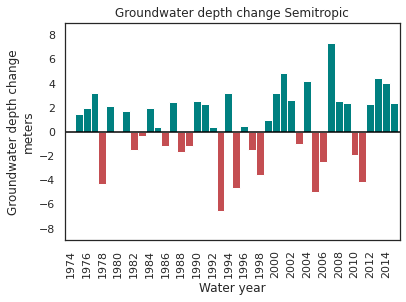
\includegraphics[width=0.6\textwidth]{Depth_change_semitropic}
    \label{fig:mesh1}
    \caption{Changes on distance to groundwater depth from C2VSIM-FG}
\end{figure}

We used Bayesian linear regression to simulate the groundwater depth response to agricultural pumping. We used C2VSIM-FG (\cite{dwr_c2vsimfg_2021}) simulation outputs from 1973 to 2015, from which we used the Groundwater Pumping at the beginning and end of each water year t ($GWP_{t}$) to predict the groundwater depth change at the end of the irrigation season in a year ($\Delta{GWD}$) as a function of the total agricultural pumping in year t $GWP_t$ and t-1 $GWP_{t-1}$. Additionally, we include Water year Type of year t ($WY_{t}$) and Water Year type of year t-1 ($WY_{t-1}$) as index variables. The water year type categories are: Wet, Normal and Dry. Normal category includes above and bellow normal categories and Dry water year includes Critical and Dry types, all of them are defined by the Water Year Hydrologic Classification Indices of the California Department of Water Resources (\cite{dwr_california_2020}). As shown by (\cite{macewan_hydroeconomic_2017}), using the water type variable we can capture information related to hydro-logical processes that shift how agricultural pumping affect groundwater depth levels.

Using groundwater pumping of the year $t$ and $t-1$ and water year type (Wet, Normal and Dry) of the year $t$ and $t-1$ as index variables we fitted different Bayesian linear modes. Pooled model (or fixed-effects) assigns same model parameters (intercept and slopes) across water year types. Un-pooled model assigns different parameters to each water year type as if water-year type is independent and have different intercepts and slopes. Finally, the Hierarchical model (or random-effects or multi-level) assigns different parameters to each water-year type varying intercepts or slopes (or both) across water-year type categories, this models enables the statistical model to learn how the agricultural pumping affects the groundwater depth change in each water year type while learning this effect from all the water wear types at the same time. 

Groundwater pumping ($GWP_{t}$, $GWP_{t-1}$) and change of depth to groundwater ($\Delta{GWD}_t$) were normalized using the z-score normalization. Bayesian modeling uses a maximum entropy distribution to define the likelihood of the output, for this study we use Student's-t distribution to model the groundwater depth change probability distribution. The characteristics of the Student's t distribution makes it a more robust distribution to include extreme values and that can improve the MCMC sampling process. Additionally we need to define priors of the parameters (or unobserved variables). For this study we defined Gaussian priors for the intercept and slopes in all the model variations. As we expect that the relationship between groundwater depth change and change being positive for which case we centered the Gaussian distribution on the positive side for ${GWP}_t$ and a less informative distribution centered in 0 for ${GWP}_{t-1}$. Additionally an exponential distribution for the standard deviation priors  and Gamma distribution for the degrees of freedom of the Student-t's distribution prior. 

\begin{itemize}[noitemsep,topsep=4pt]
  \item P1: Pooled,   $\mu_t = \alpha + \beta_{1}GWP_{t}$
  \item P2: Pooled with lag on pumping,   $\mu_t = \alpha + \beta_{1}GWP_{t} + \beta_{2}GWP_{t-1} $
  \item U1: Unpooled, $\mu_t = \alpha_{WY_{t}} + \beta_{1,WY_{t}}GWP_{t}$
  \item U2: Unpooled with lag on pumping, $\mu_t = \alpha_{WY_{t}} + \beta_{1,WY_{t}}GWP_{t} + \beta_{2,WY_{t}}GWP_{t} $
  \item U3: Unpooled with lag on pumping and slope, $\mu_t =  \alpha_{WY_{t}} + \gamma_{WY_{t-1}} + \beta_{1,WY_{t}}GWP_{t} + \beta_{2,WY_{t}}GWP_{t}$
  \item H1: Hirerarchical with varying intercept, $\mu_t = \alpha_{WY_{t}} + \beta_{1}GWP_{t}$
  \item H2: Hirerarchical with varying intercept and varying slope, $\mu_t = \alpha_{WY_{t}} + \beta_{1,WY_{t}}GWP_{t}$
  \item H3: Hirerarchical with varying slopes, $\mu_t = \alpha_t + \beta_{1,WY_{t}}GWP_{t} + \beta_{2,WY_{t}}GWP_{t}$
  \item H4: Hirerarchical with varying intercept and slopes, $\mu_t = \alpha_{WY_{t}} + \beta_{1,WY_{t}}GWP_{t} + \beta_{2,WY_{t}}GWP_{t}$
  \item H5: Hirerarchical with varying intercepts and slopes, $\mu_t = \alpha_{WY_{t}} + \gamma_{WY_{t-1}} + \beta_{1,WY_{t}}GWP_{t} + \beta_{2,WY_{t}}GWP_{t}$
\end{itemize}

Models were fit using a Markov Chain Monte Carlo (MCMC) sampling method using the probabilistic programming Python package PyMC (\cite{salvatier_probabilistic_2016}). Model selection was done using the Leave-one-out Cross-validation (LOO-CV) as estimate of the out-of-sample predictive fit (\cite{vehtari_practical_2017}), selecting the model with the highest log-scale LOO-CV or with he best out-of-sample prediction (Figure S3). The LOO-CV validation results are summarized in the Figure S8. Where the best model is the hirerarchical model with varying intercepts (H5), however the model with unpooled effects in intercepts and pumping (U3) was selected since is a simpler model and has a LOO close to H5. Hence, obtaining similar predictive power for a more computational efficient model. 

\begin{figure}[H]
\centering
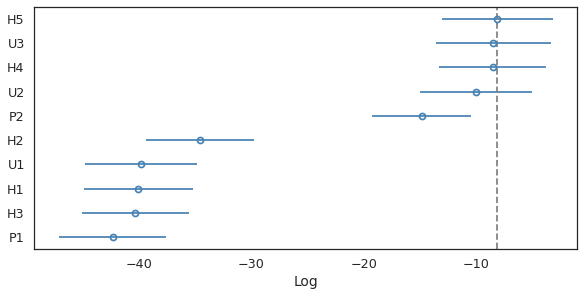
\includegraphics[width=0.7\textwidth]{model_comparison_calibration.png}
\label{fig:mesh1}
\caption{Leave-one-out cross-validation results}
\end{figure}

The selected model is an unpooled model with priors defined in Equations B.1. Table S1 shows the results from the model U3 summarizing the distribution of the posterior distribution of the parameters. In Figure B.1 we show that calibrated response function can predict correctly the groundwater depth change with an $r^2 = 0.90 (r^2 std = 0.007)$. 

\begin{figure}[H]
\centering
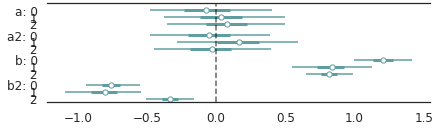
\includegraphics[width=0.7\textwidth]{gw_depth_response_posterior_2.png}
\label{fig:mesh1}
\caption{Posterior Distributions of the parameters, where 0 is Wet Year, 1 is Normal Year and 2 is Dry Year}
\end{figure}

\begin{align}
\Delta & GWD_{t} \sim Student \mh t(\mu_{t},\sigma,\nu) & \notag\\
\mu_t & = \alpha_{WY_{t}} +  \gamma_{WY_{t-1}} + \beta_{1  WY_{t}}GWP_{t} + \beta_{2  WYR_{t-1}} GWP_{t-1} \notag\\
\alpha_j & = Normal(0 ,0.5)\notag\\
\gamma_j & = Normal(0,0.5)\\
\beta_{1j} & = Normal(0.5,0.5) \hspace{1em}  for j = \{Wet,Normal,Dry\} \notag\\
\beta_{2j} & = Normal(0,0.5) \notag\\
\sigma & = Exponential(1) \notag\\
\nu & = Gamma(2,0.1)\notag
\end{align}

\begin{center}
\begin{tabular}{ |c|c|c|c|c| }
 \hline
 Parameter & Mean & Sd & HDI $2.5\%$ & HDI $97.5\%$ \\ 
 \hline
$\alpha_{1[Wet_{t}]}$ & 	-0.063 &	0.232 &	-0.478 &	0.405 		 \\
$\alpha_{1[Normal_{t}]}$ & 0.041 &	0.223 &	-0.379 &	0.501 	 \\
$\alpha_{1[Dry_{t}]}$ & 	 0.079 &	0.217 &	-0.356 &	0.494	 \\
$\gamma_{1[Wet_{t}]}$ & 	-0.057 	& 0.224 &	-0.481 &	0.393 	 \\
$\gamma_{1[Normal_{t}]}$ & 0.159 &	0.225 &	-0.285 &	0.588 \\
$\gamma_{1[Dry_{t}]}$ & -0.041 &	0.217 &	-0.453 &	0.400 	 \\
$\beta_{1[Wet_{t \mh 1}]}$ & 1.207 &	0.107 &	0.995 &	1.419 	 \\
$\beta_{1[Normal_{t \mh 1}]}$ 	& 0.829 &	0.148 &	0.550 &	1.126	\\
$\beta_{1[Dry_{t \mh 1}]}$ & 0.817 &	0.088 &	0.649 &	0.991 \\
$\beta_{2[Wet_{t \mh 1}]}$ & -0.757 	& 0.100 & -0.940 & 	-0.551 	 \\
$\beta_{2[Normal_{t \mh 1}]}$ & -0.807 &	0.141 &	-1.094 & -0.543 	\\
$\beta_{2[Dry_{t \mh 1}]}$ & -0.336 	& 0.088 & 	- 0.507 &  -0.159 \\
$\sigma$ & 0.235 & 	0.037 & 0.169 & 	0.310 \\
$\nu$ 	& 20.470 & 	12.859 & 2.469 &  	45.244 \\
\hline
\end{tabular}
\captionof{table}{Marginal posterior distributions of the parameters of Groundwater Depth Response}
\end{center}

\begin{figure}[H]
    \centering
    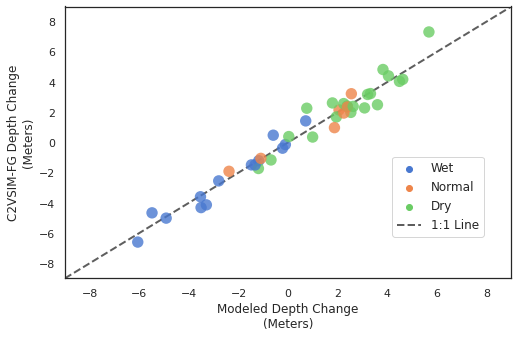
\includegraphics[width=0.6\textwidth]{results_gw_depth_response_calib.png}
    \caption{Results groundwater depth response function and C2VSIM-FG (\cite{dwr_c2vsimfg_2021}). Dots represent the median of each posterior predictive distribution of groundwater depth change, colors represent the water-year type in year t.}
    \label{fig:mesh1}
\end{figure}

\section{Calibrated Hydro-Economic Model Performance}

The following figures show the performance from running dynamically the coupled hydro-economic model with the last set of calibration parameters obtained from the data assimilation process (with 400 samples) over historical water available conditions. The model was let free to optimize dynamically land and water allocation decisions to assess its capacity to replicate observed conditions. 

\begin{figure}[H]
\centering
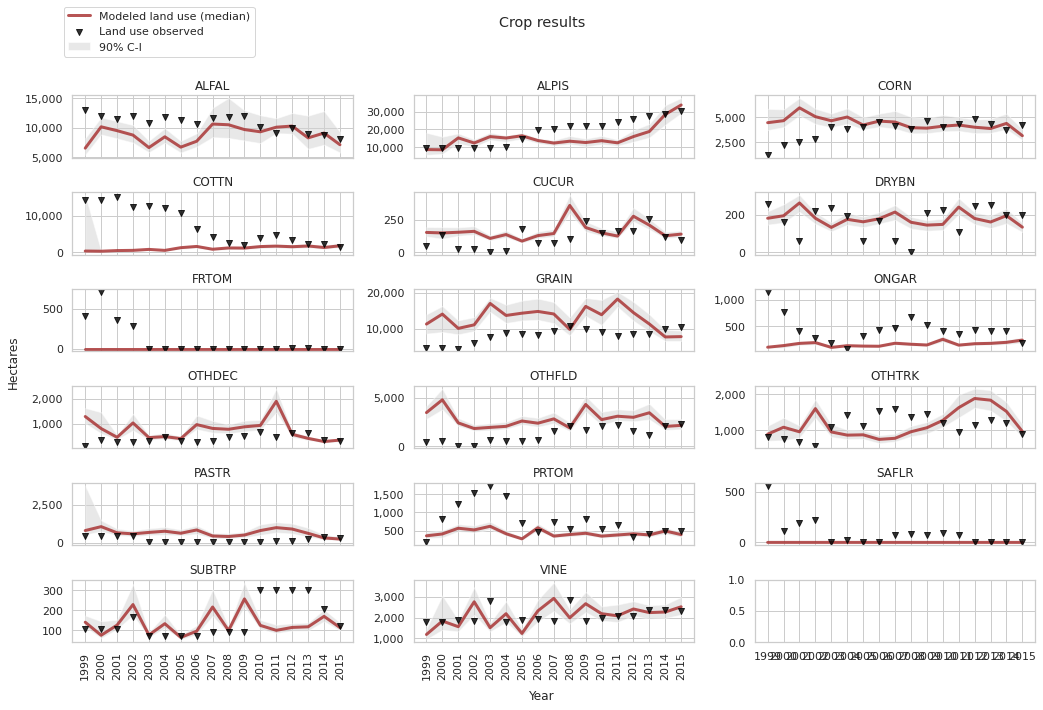
\includegraphics[width=1\textwidth]{./figs/land_use.png}
\label{fig:mesh1}
\caption{Land allocation from Hydro-economic model and observed}
\end{figure}

\begin{figure}[H]
\centering
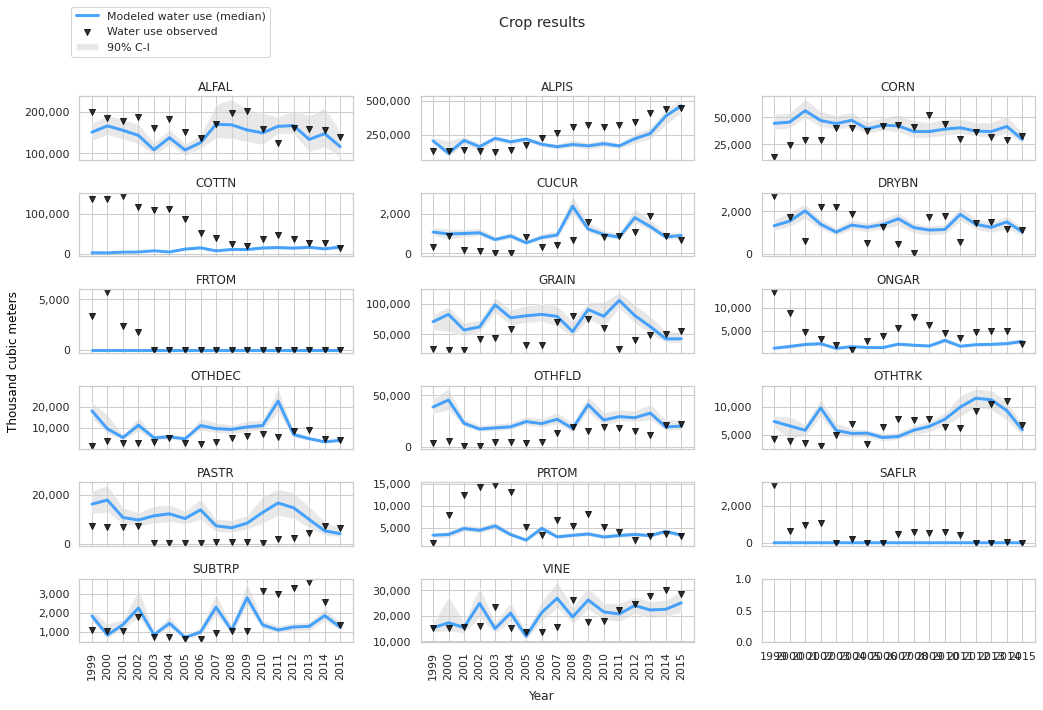
\includegraphics[width=1\textwidth]{./figs/water_use.png}
\label{fig:mesh1}
\caption{Water allocation from Hydro-economic model and observed}
\end{figure}

\begin{figure}[H]
\centering
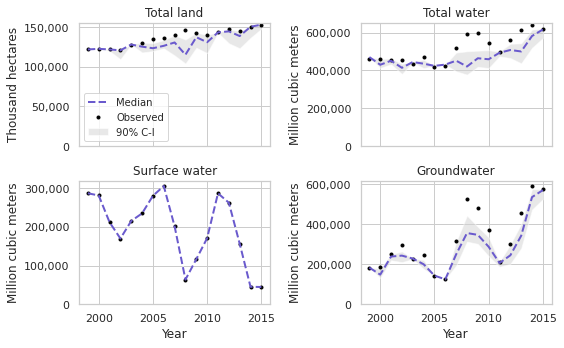
\includegraphics[width=0.8\textwidth]{./figs/water_use_by_source.png}
\label{fig:mesh1}
\caption{Total water allocation by source from Hydro-economic model and observed}
\end{figure}

\begin{figure}[H]
\centering
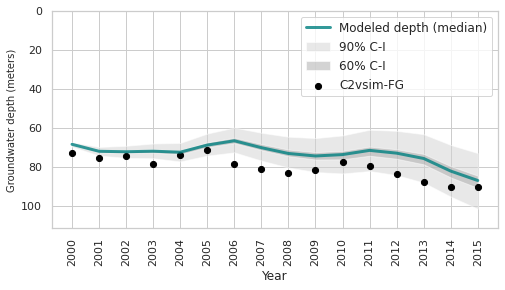
\includegraphics[width=0.6\textwidth]{./figs/gw_depth.png}
\label{fig:mesh1}
\caption{Simulated groundwater depth from running coupled hydro-economic model dynamically  and observed groundwater depth from \textcite{dwr_c2vsimfg_2021}}
\end{figure}


\section{Surface Water Deliveries used in Computational Experiment}

\begin{figure}[htb!]
    \centering
    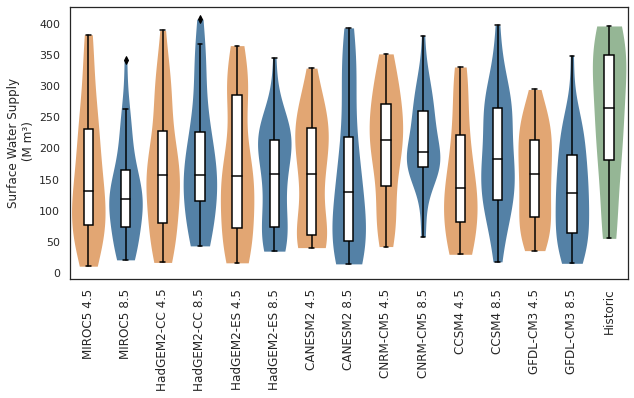
\includegraphics[width=0.7\textwidth]{./figs/gcm_surface_water.png}
    \caption{Distribution of historical (1999-2015) and surface water deliveries from CALFEWS (2016-2045) used in this study} \label{fig:SWSemitropic}
\end{figure}



\section{Borg Epsilon values and Hypervolume from Random Seeds}

\begin{center}
\begin{tabular}{ |c|c| }
 \hline
 Objective & Epsilon \\ 
 \hline
Maximize Average Total Revenues (O1) & 30  \\
Minimize Average Groundwater Depth (O2) & 1.8 \\
Maximize 5th Percentile Revenue in a year (O3) & 1 \\
Minimize 95th Groundwater Depth Change in a year (O4) & 0.9 \\
Reliability (O5) & 0.01 \\
\hline
\end{tabular}
\captionof{table}{Epsilon values used for the Borg MOEA}
\end{center}

\begin{figure}[H]
    \centering
    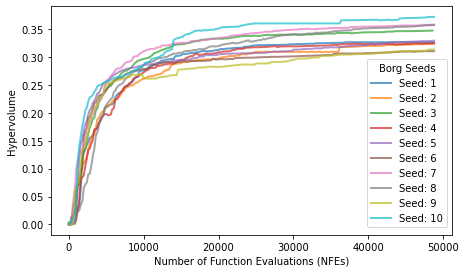
\includegraphics[width=0.9\textwidth]{./figs/Borg_Seeds_Hypervolume.png}
    \caption{Hypervolume from 10 random seeds used in Borg MOEA}
    \label{fig:m1esh1}
\end{figure}

\section{Pareto-approximate set validation}

\begin{figure}[H]
    \centering
    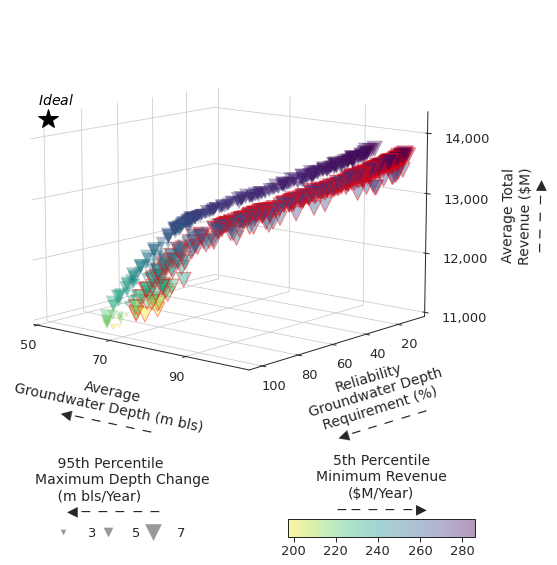
\includegraphics[width=0.9\textwidth]{./figs/validation_pareto_set.png}
    \caption{Reference pareto set was re-evaluated using a larger independent set of 1,000 sets of sampled SOWs. Triangles with red edge represent the re-evaluated set and triangles without edge the original optimized solution.}
    \label{fig:m1esh1}
\end{figure}

\section{Performance selected Policies}

The following figures show the performance of the selected solutions in Section 5.

\begin{figure}[H]
    \centering
    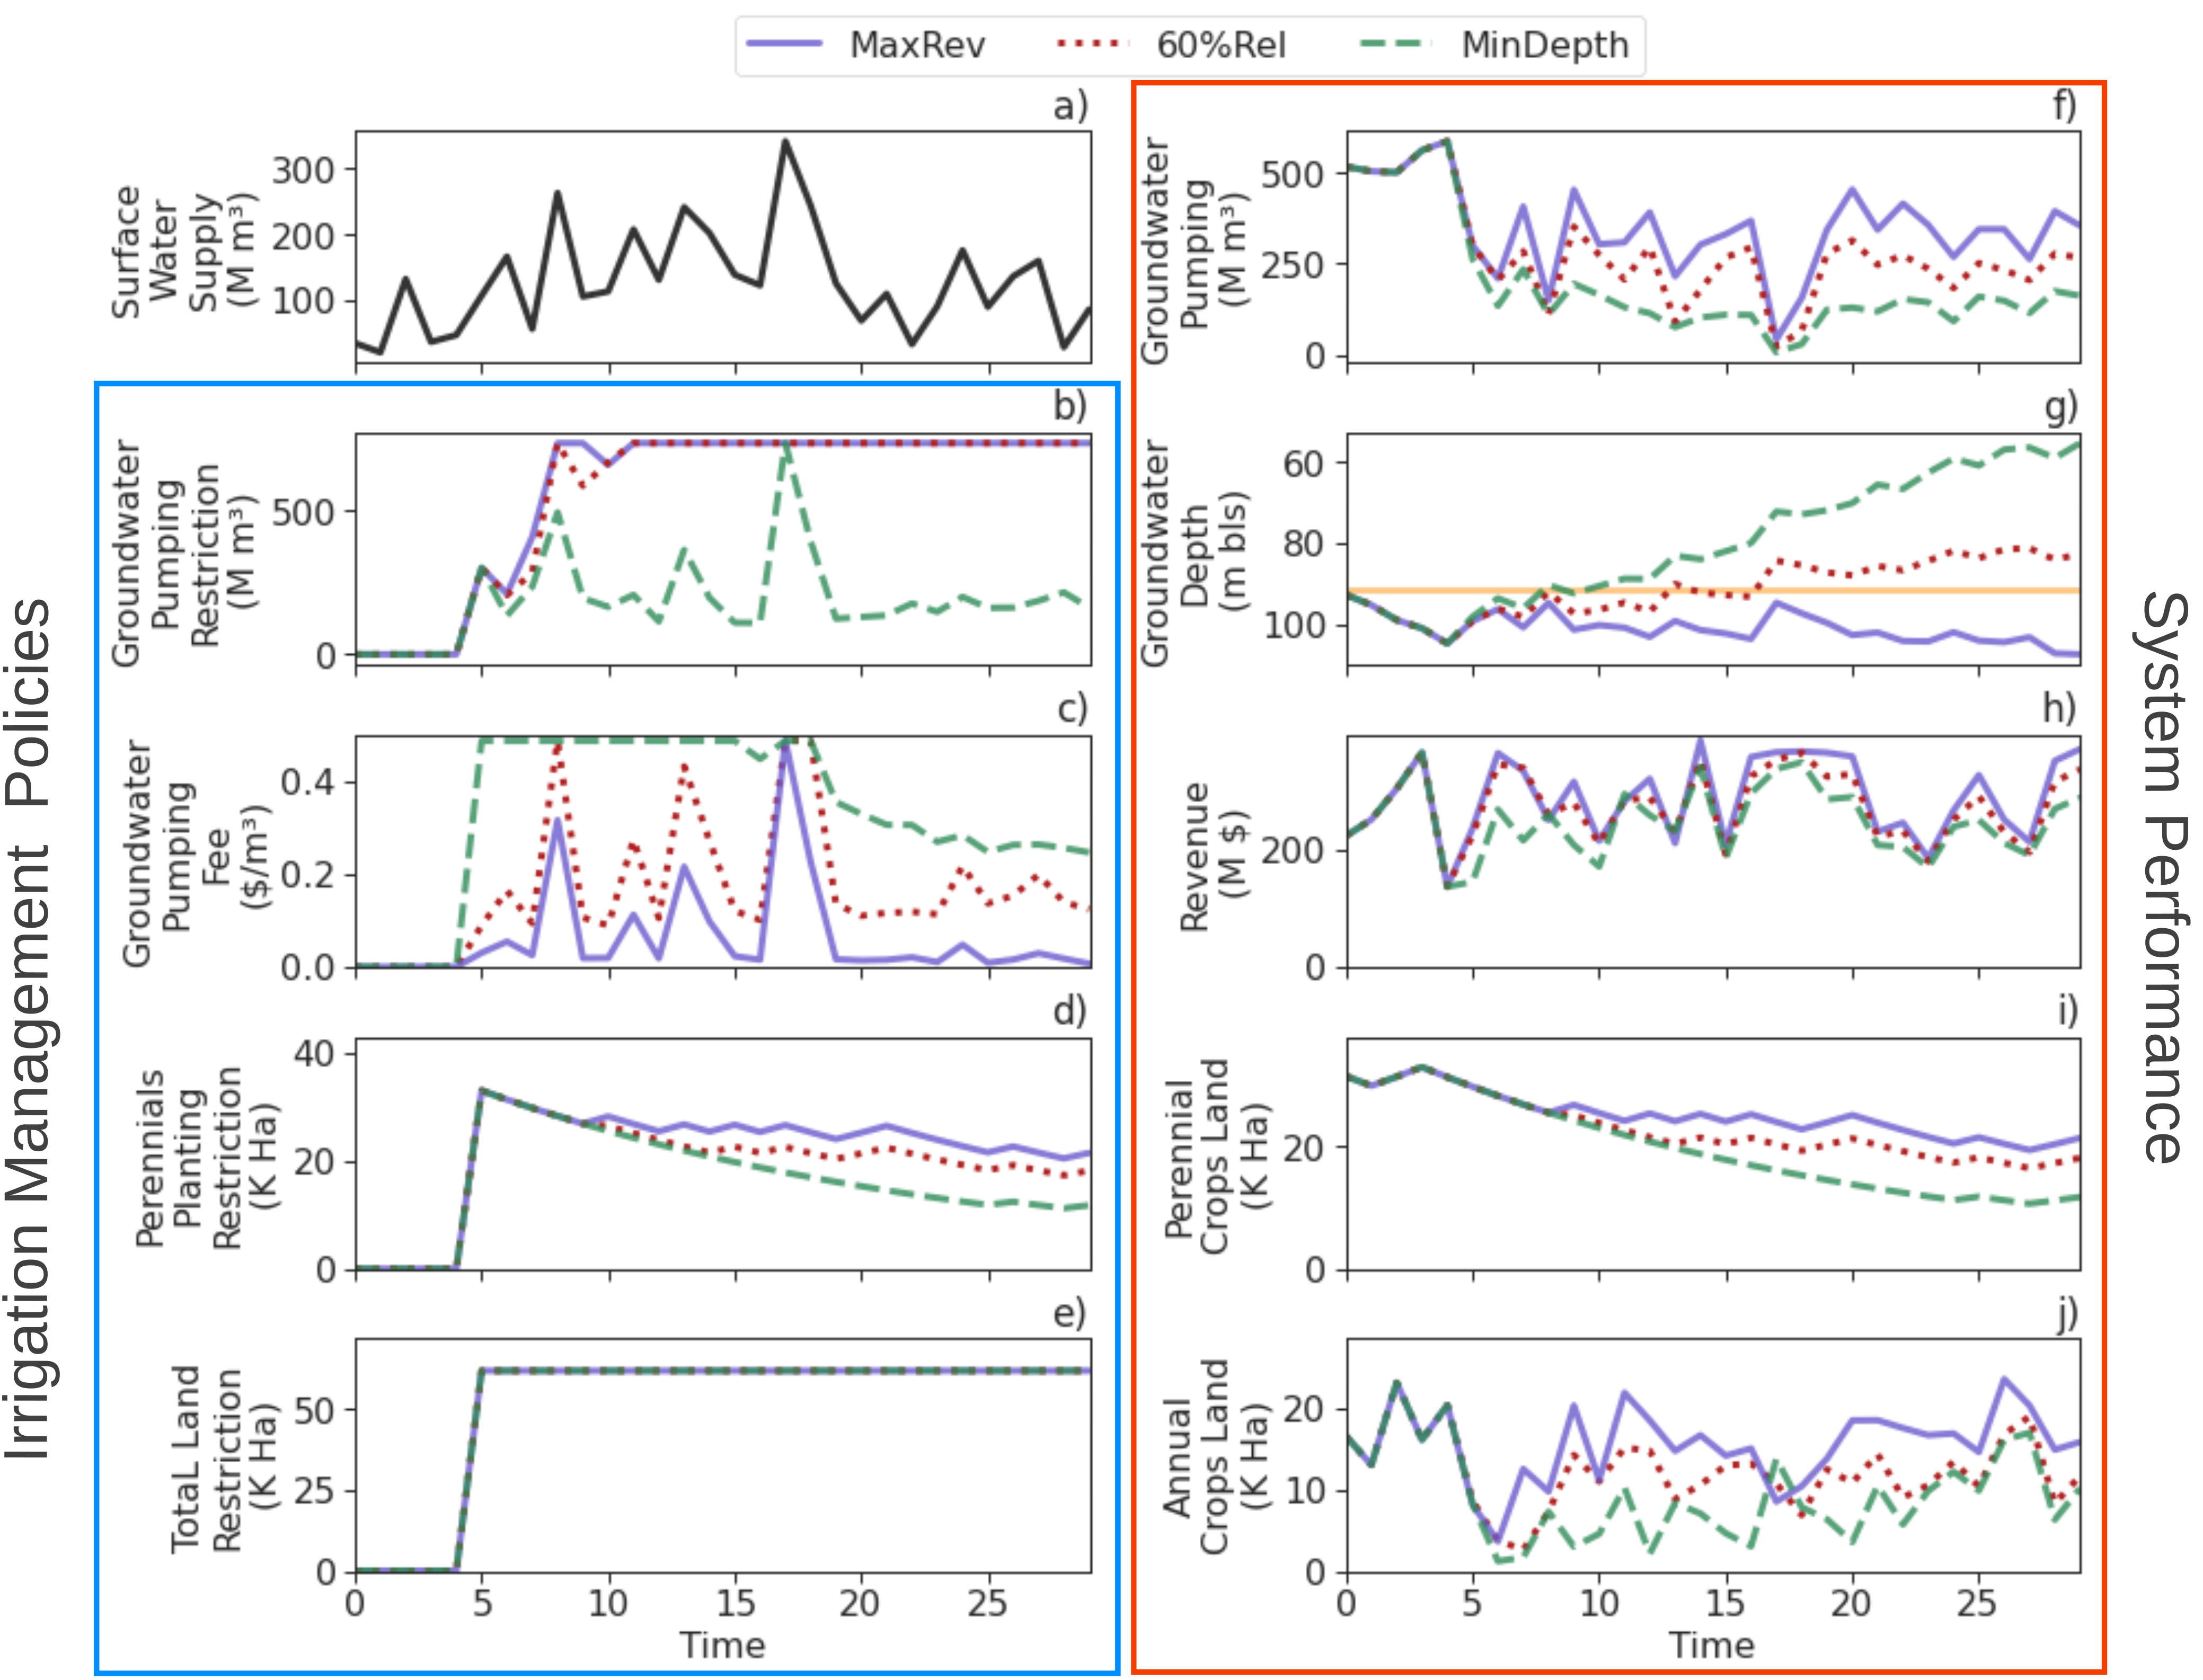
\includegraphics[width=1\textwidth]{./figs/selected_dry_performance.png}
    \caption{Performance selected policies, shown in Figure 5, under driest average surface water deliveries (MIROC 8.5). Panel (a) shows the surface water deliveries. Panels (b) - (e) show the dynamic decisions in the control policy. Panels (f)-(j) show the performance of the food-water system. The orange line in Sub-figure (g) depicts the measurable objective used in the experiment}
    \label{fig:m1esh1}
\end{figure}



\begin{figure}[H]
    \centering
    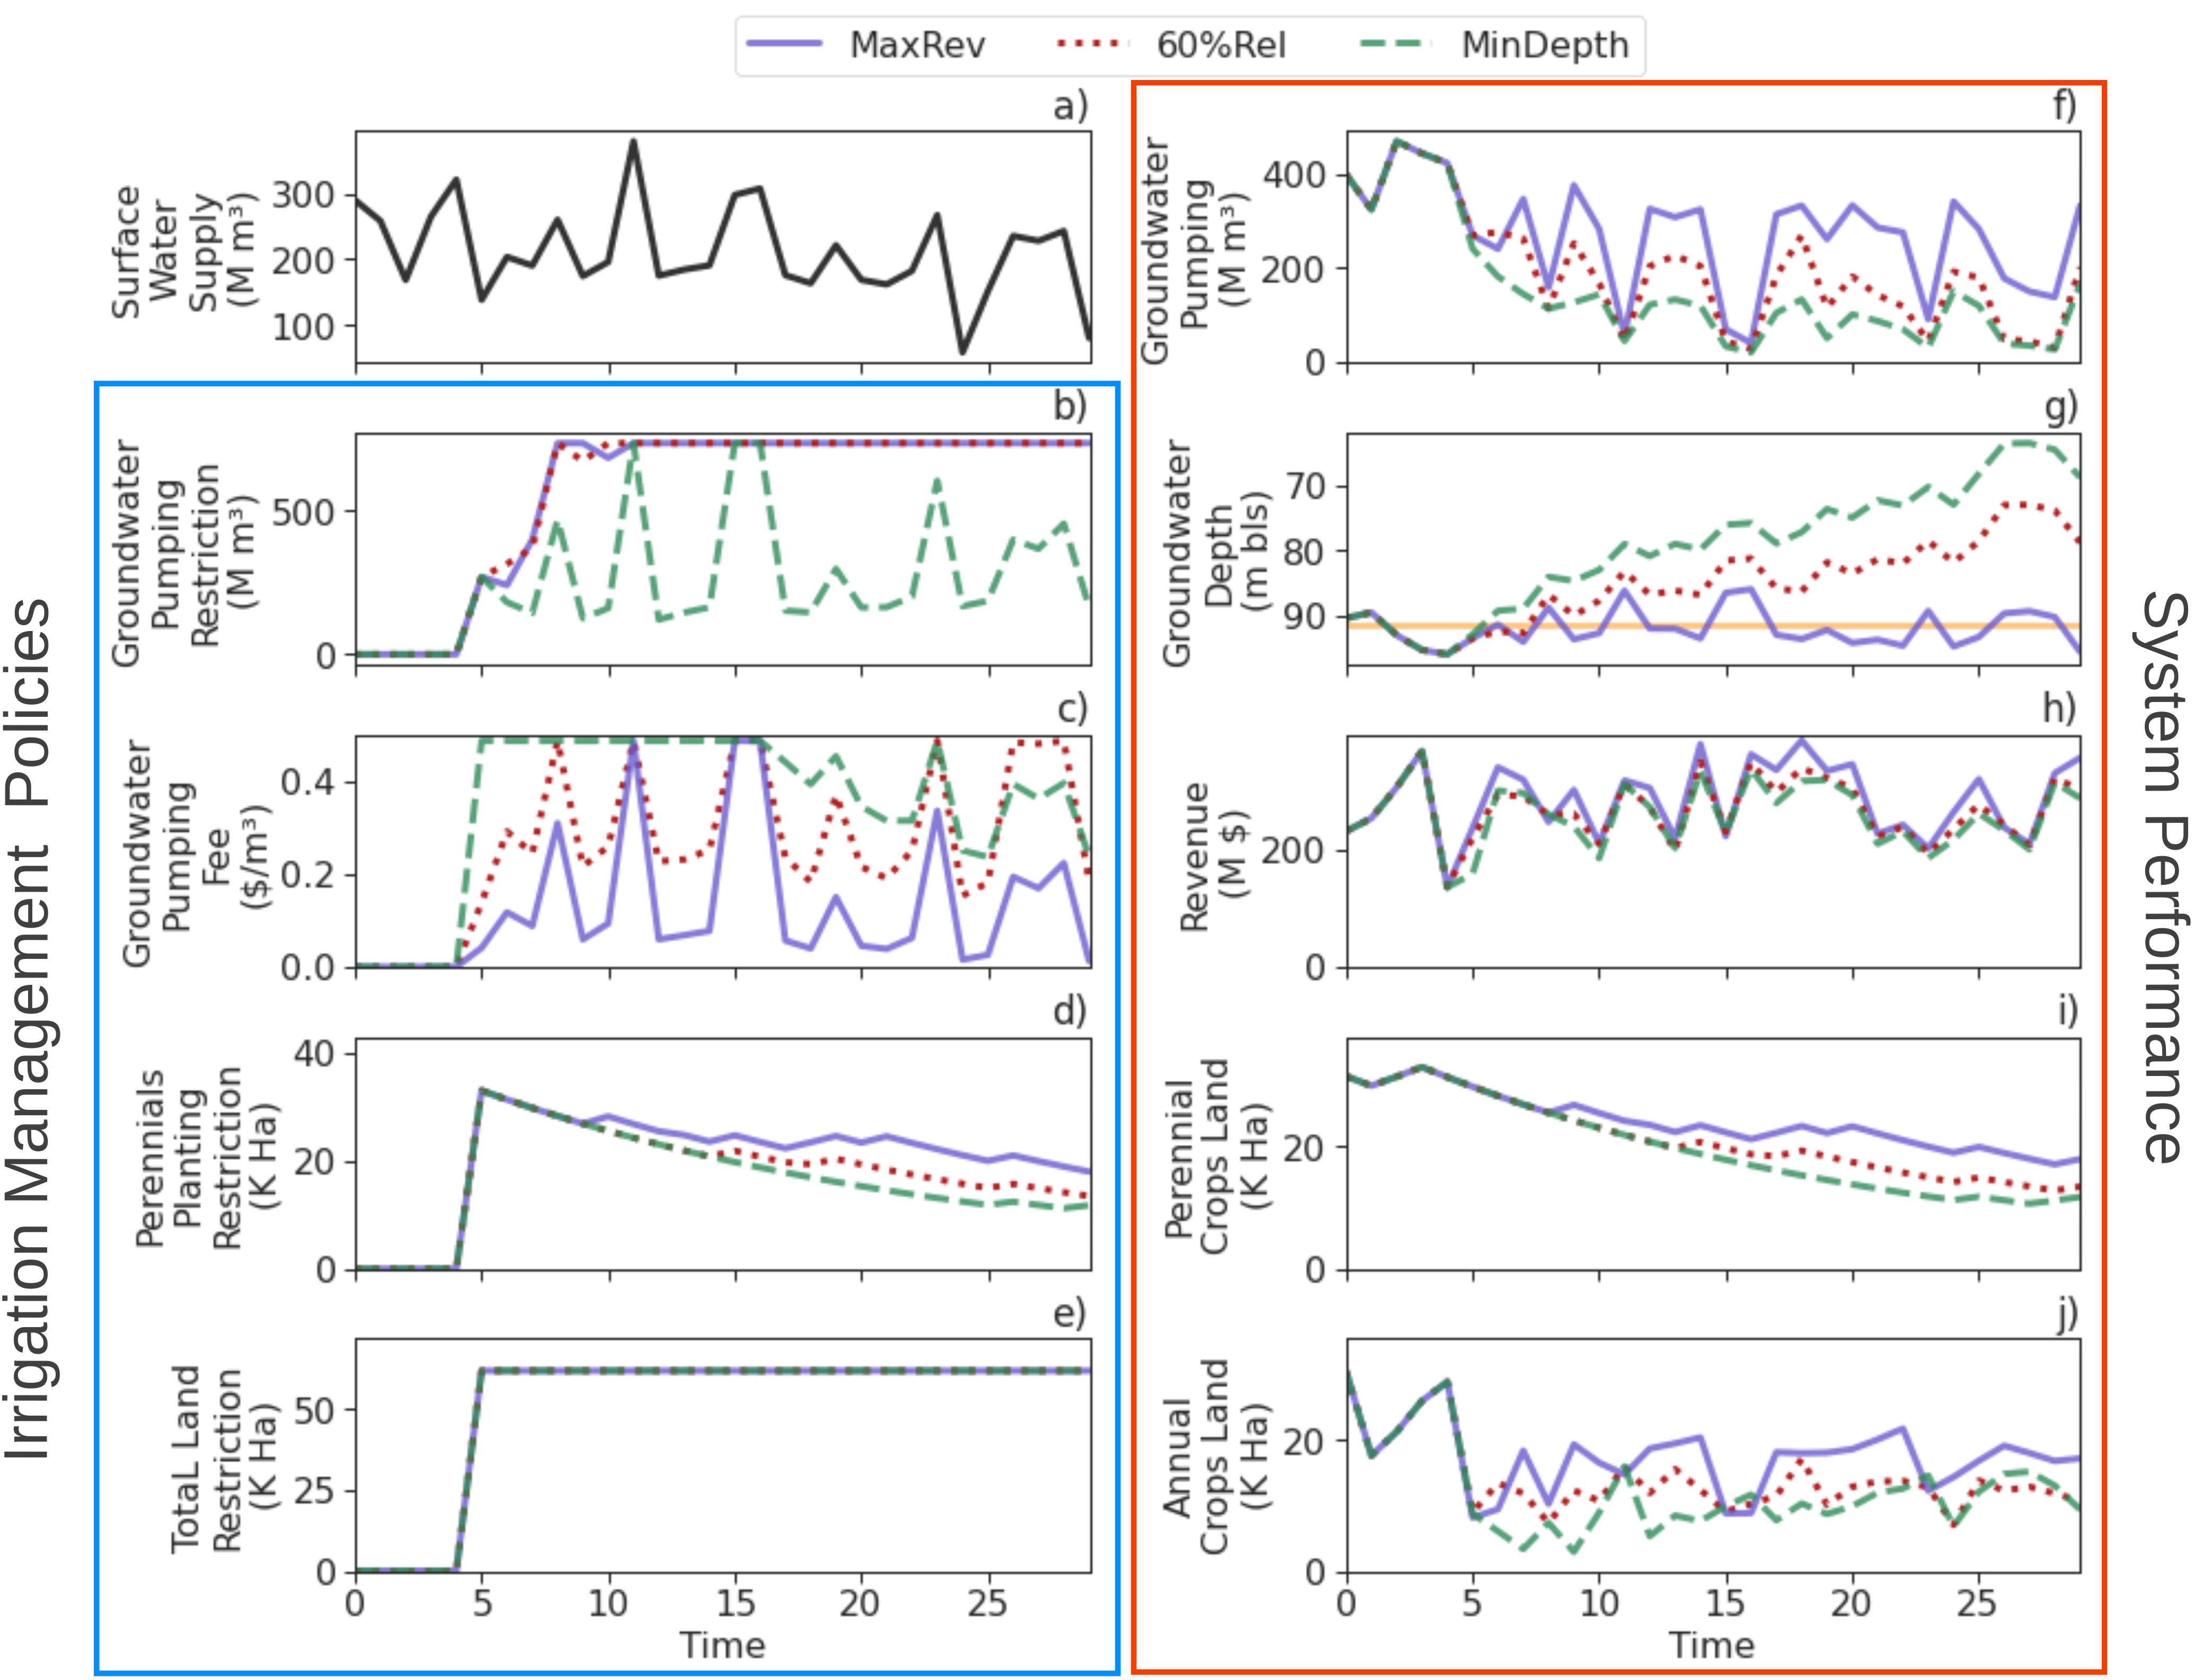
\includegraphics[width=1\textwidth]{./figs/selected_wet_performance.png}
    \caption{Performance selected policies, shown in Figure 5, under largest (wet) average surface water deliveries (CNRM-CM5 8.5). Panel (a) shows the surface water deliveries. Panels (b) - (e) show the dynamic decisions in the control policy. Panels (f)-(j) show the performance of the food-water system. The orange line in Sub-figure (g) depicts the measurable objective used in the experiment}
    \label{fig:m1esh1}
\end{figure}

\section{Performance selected Robust Policies}

The following figures show the performance of the selected robust solutions in Section 5.1



\begin{figure}[H]
    \centering
    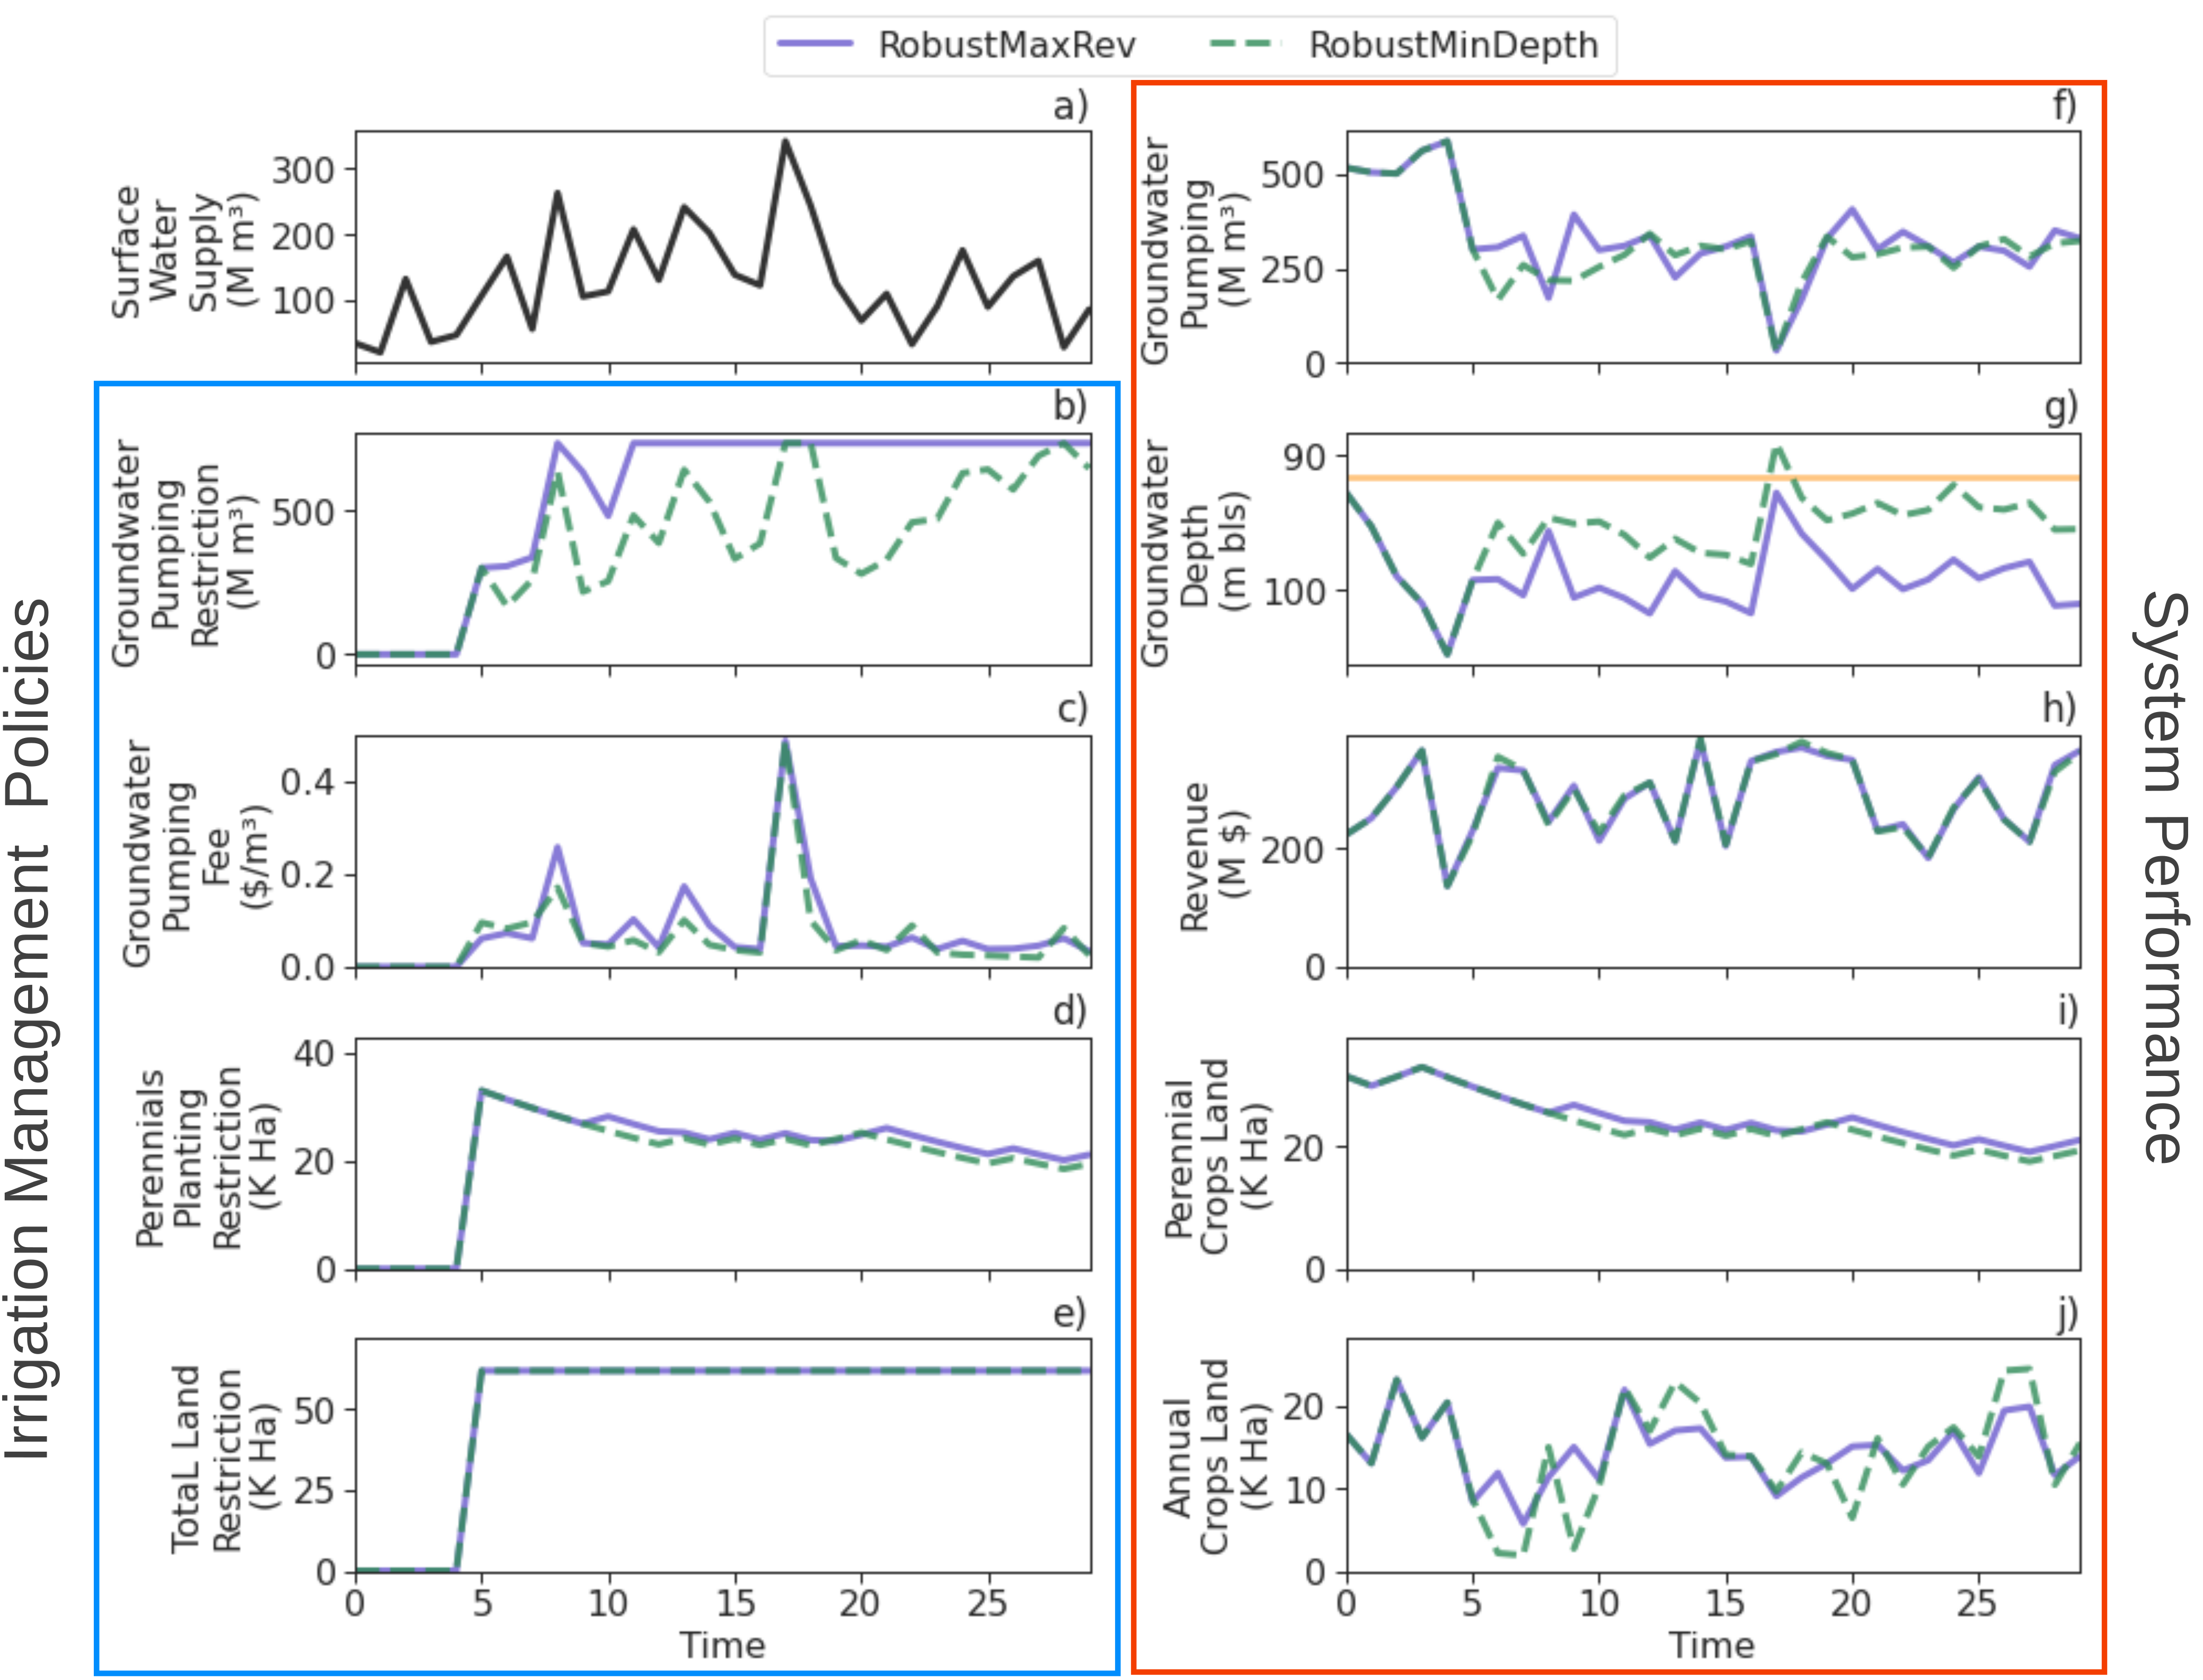
\includegraphics[width=1\textwidth]{./figs/robust_dry_performance.png}
    \caption{Performance Robust Policy under driest average surface water deliveries (MIROC 8.5). Panel (a) shows the surface water deliveries. Panels (b) - (e) show the dynamic decisions in the control policy. Panels (f)-(j) show the performance of the food-water system. The orange line in Sub-figure (g) depicts the measurable objective used in the experiment}
    \label{fig:m1esh1}
\end{figure}



\begin{figure}[H]
    \centering
    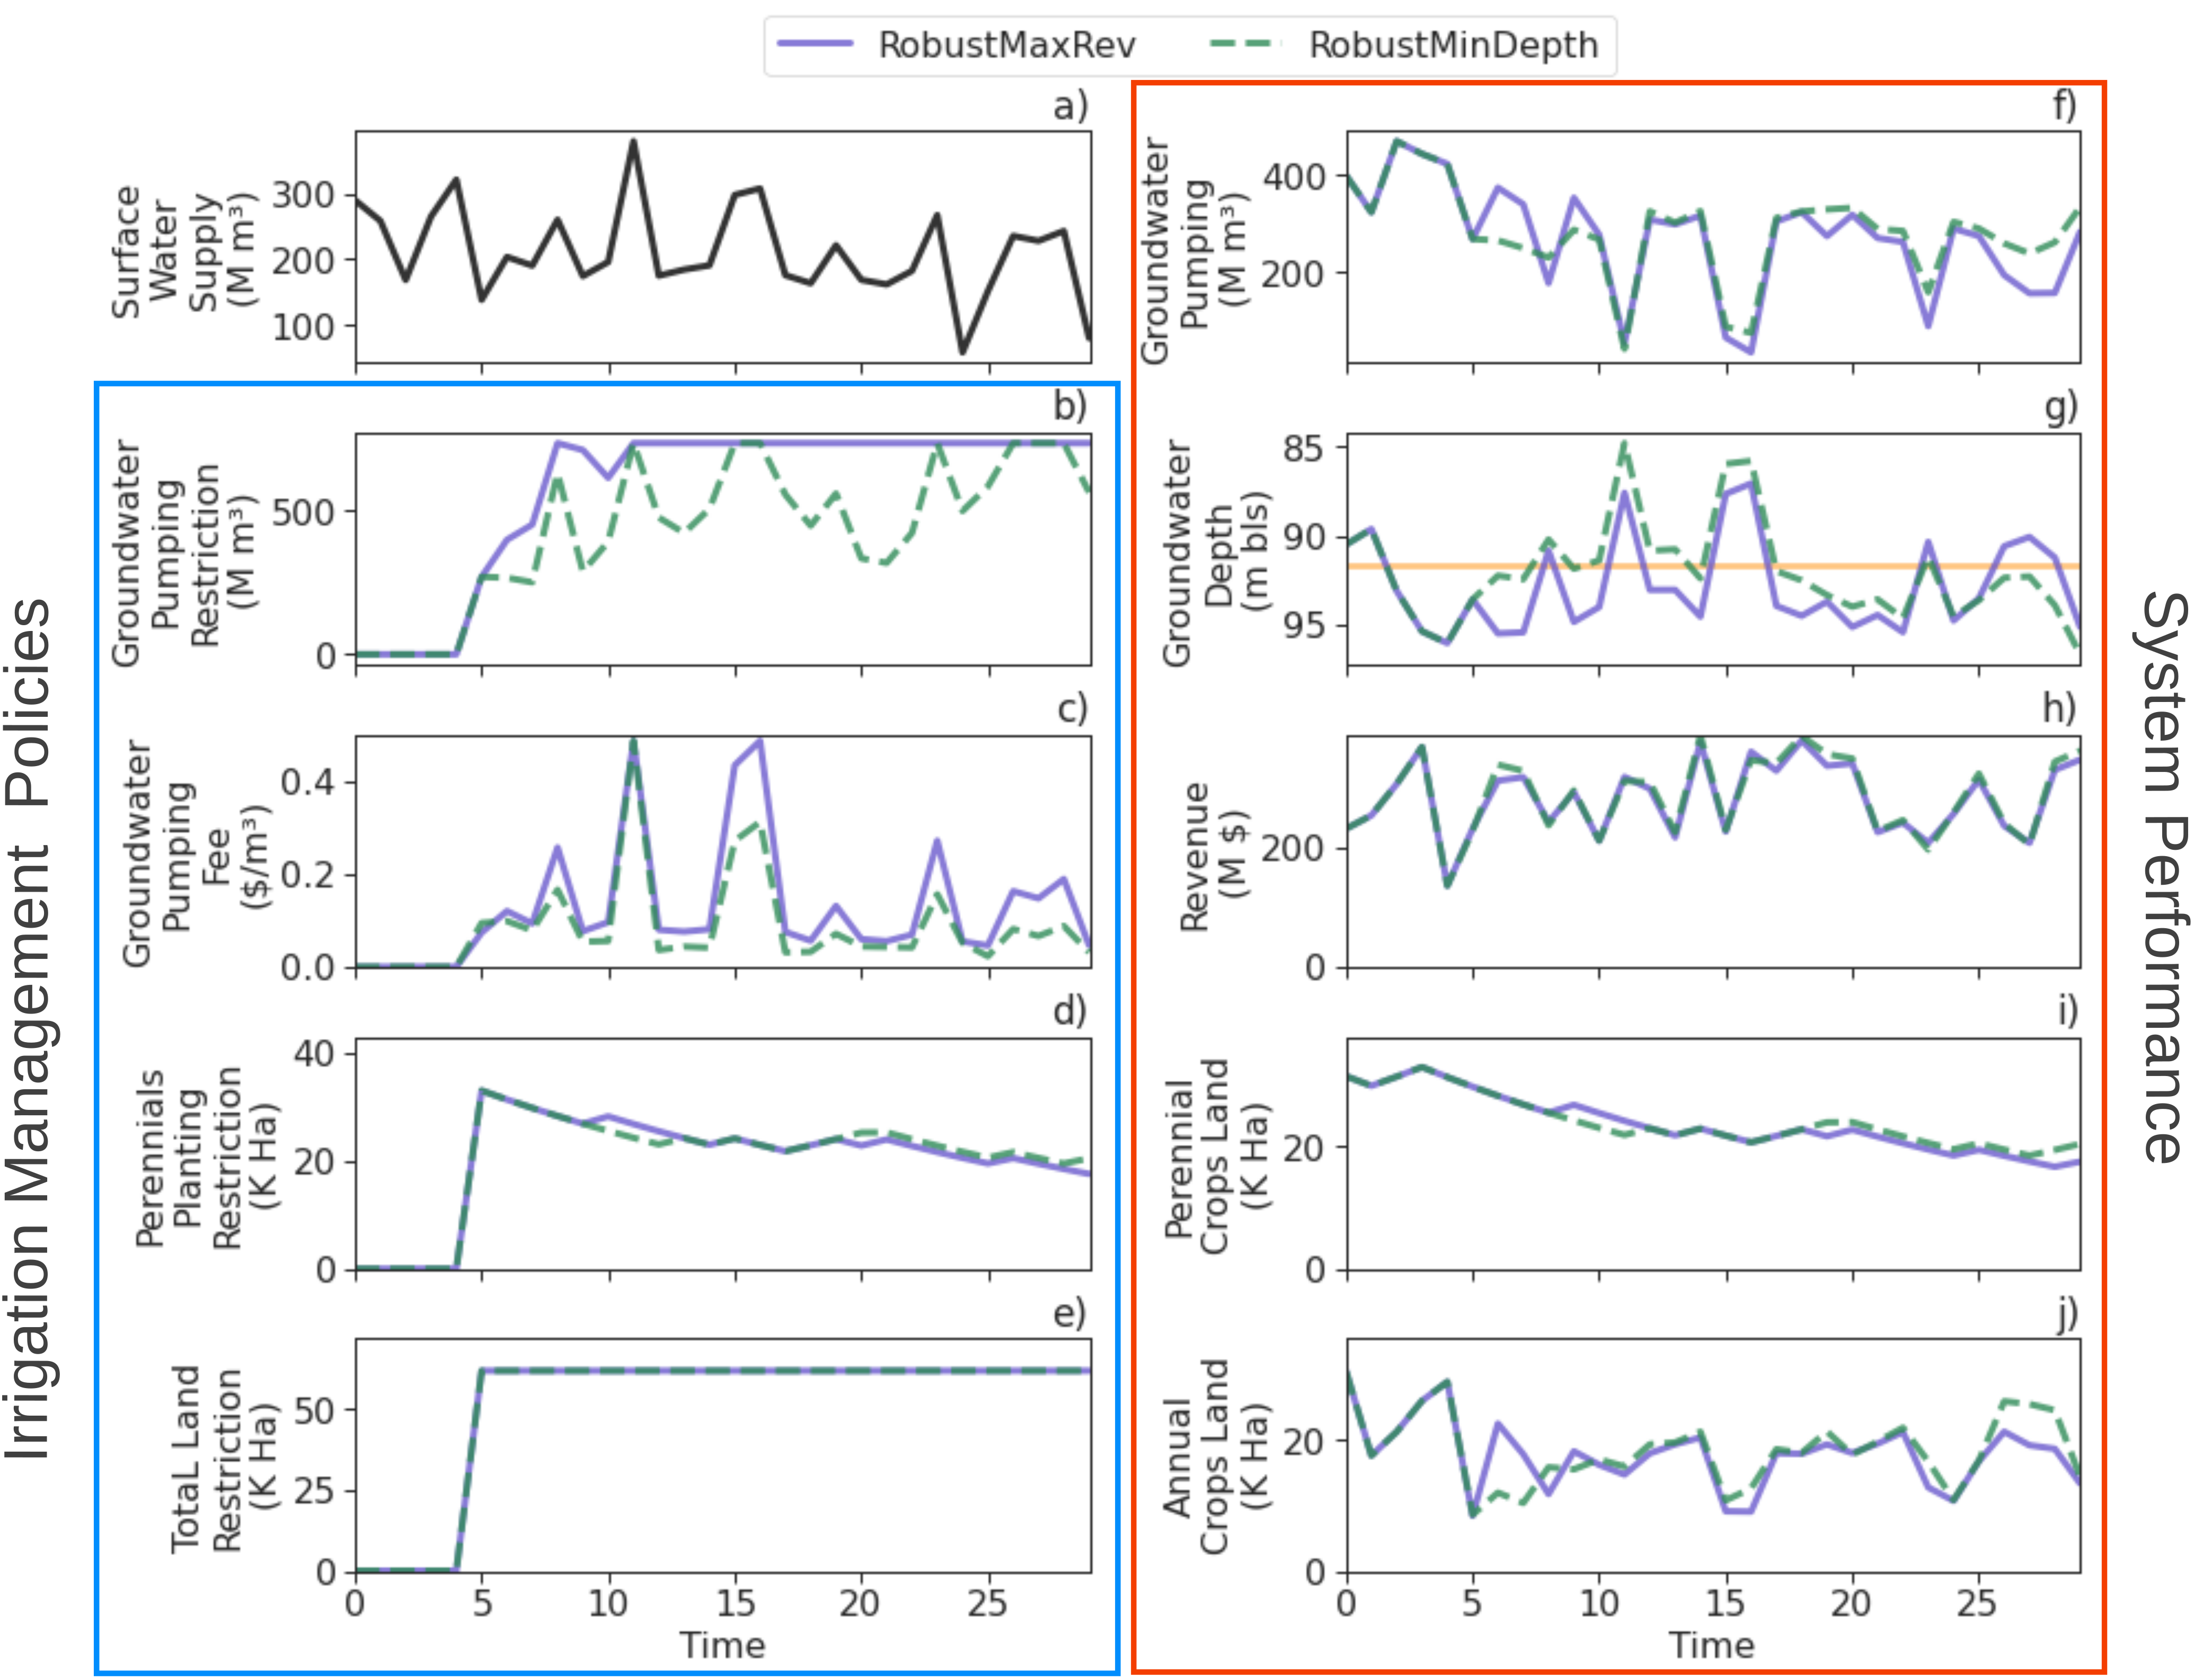
\includegraphics[width=1\textwidth]{./figs/robust_wet_performance.png}
    \caption{Performance Robust Policy under largest (wet) average surface water deliveries (CNRM-CM5 8.5). Panel (a) shows the surface water deliveries. Panels (b) - (e) show the dynamic decisions in the control policy. Panels (f)-(j) show the performance of the food-water system. The orange line in Sub-figure (g) depicts the measurable objective used in the experiment}
    \label{fig:m1esh1}
\end{figure}

\section{Feature Scoring}

\begin{figure}[H]
    \centering
    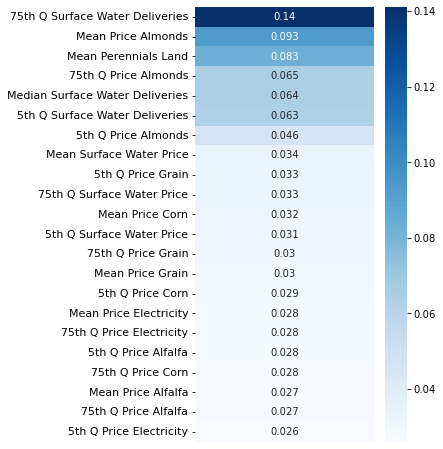
\includegraphics[width=0.7\textwidth]{./figs/prim_robust_mindepth_rank.png}
    \caption{Feature Scoring for the RobustMinDepth solution}
    \label{fig:m1esh1}
\end{figure}

\begin{figure}[H]
    \centering
    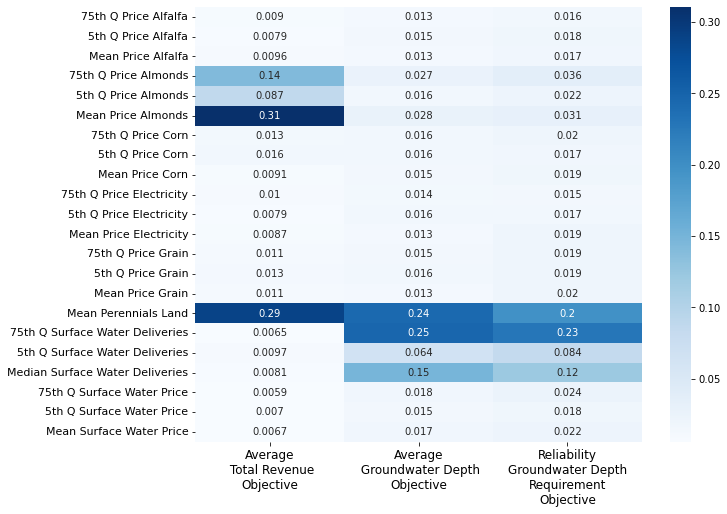
\includegraphics[width=0.9\textwidth]{./figs/prim_robust_mindepth_rank_objectives.png}
    \caption{Feature Scoring for the RobustMinDepth solution for each objective}
    \label{fig:m1esh1}
\end{figure}

\newpage
\printbibliography

\end{document}
